% ****************************************************************************************** % Dissertation template and document class for Princeton University
% Author  : Jeffrey Scott Dwoskin <jdwoskin@princeton.edu>
% Adapted from: http://www.math.princeton.edu/graduate/tex/puthesis.html
% ****************************************************************************************** %


%%% For print copies
%% set 'singlespace' option to set entire thesis to single space, and define "\printmode" to remove all hyperlinks for printed copies of the thesis. Delete all output files before changing this mode -- it will turn hyperref package on and off
%\documentclass[12pt,lot, lof, singlespace]{puthesis}
%\newcommand{\printmode}{}

%%% For the electronic copy, use doublespacing, define "\proquestmode" to use outlined links, instead of colored links. 
\documentclass[12pt,lot, lof]{puthesis}
\newcommand{\proquestmode}{}
% I prefer proquestmode to be off for electronic copies for normal use, since the colored links are less distracting. However when printed in black and white, the colored links are difficult to read. 

%%% For early drafts without some of the frontmatter
% Also see the "ifodd" command below to disable more frontmatter
%\documentclass[12pt]{puthesis}

%%%%%%%%%%%%%%%%%%%%%%%%%%%%%%%%%%%%%%%%%%%%%%%%%%%%%%%%%%%%%\
%%%% Author & title page info

\title{Dissertation Template for Princeton University}

\submitted{June 2010}  % degree conferral date (January, April, June, September, or November)
\copyrightyear{2010}  % year in which the copyright is secured by publication of the dissertation.
\author{First Middle Last}
\adviser{Professor Smith}  %replace with the full name of your adviser
%\departmentprefix{Program in}  % defaults to "Department of", but programs need to change this.
\department{Electrical Engineering}

%%%%%%%%%%%%%%%%%%%%%%%%%%%%%%%%%%%%%%%%%%%%%%%%%%%%%%%%%%%%%\
%%%% Tweak float placements
% From: http://mintaka.sdsu.edu/GF/bibliog/latex/floats.html "Controlling LaTeX Floats"
% and based on: http://www.tex.ac.uk/cgi-bin/texfaq2html?label=floats
% LaTeX defaults listed at: http://people.cs.uu.nl/piet/floats/node1.html

% Alter some LaTeX defaults for better treatment of figures:
    % See p.105 of "TeX Unbound" for suggested values.
    % See pp. 199-200 of Lamport's "LaTeX" book for details.
    %   General parameters, for ALL pages:
    \renewcommand{\topfraction}{0.85}	% max fraction of floats at top
    \renewcommand{\bottomfraction}{0.6}	% max fraction of floats at bottom
    %   Parameters for TEXT pages (not float pages):
    \setcounter{topnumber}{2}
    \setcounter{bottomnumber}{2}
    \setcounter{totalnumber}{4}     % 2 may work better
    \setcounter{dbltopnumber}{2}    % for 2-column pages
    \renewcommand{\dbltopfraction}{0.66}	% fit big float above 2-col. text
    \renewcommand{\textfraction}{0.15}	% allow minimal text w. figs
    %   Parameters for FLOAT pages (not text pages):
    \renewcommand{\floatpagefraction}{0.66}	% require fuller float pages
	% N.B.: floatpagefraction MUST be less than topfraction !!
    \renewcommand{\dblfloatpagefraction}{0.66}	% require fuller float pages

% The documentclass already sets parameters to make a high penalty for widows and orphans. 

%%%%%%%%%%%%%%%%%%%%%%%%%%%%%%%%%%%%%%%%%%%%%%%%%%%%%%%%%%%%%\
%%%% Use packages

%\usepackage{amsfonts}

%%% For figures
\usepackage{graphicx}
%\usepackage{subfig,rotate}

%%% for comments
\usepackage{verbatim}

%%% For tables
\usepackage{multirow}
% Longtable lets you have tables that span multiple pages.
\usepackage{longtable}

% Booktabs produces far nicer tables than the standard LaTeX tables.
%   see: http://en.wikibooks.org/wiki/LaTeX/Tables
\usepackage{booktabs}

%set parameters for longtable:
% default caption width is 4in for longtable, but wider for normal tables
\setlength{\LTcapwidth}{\textwidth}



%%%%%%%%%%%%%%%%%%%%%%%%%%%%%%%%%%%%%%%%%%%%%%%%%%%%%%%%%%
%%% Printed vs. online formatting
\ifdefined\printmode

% Printed copy
% url package understands urls (with proper line-breaks) without hyperlinking them
\usepackage{url}


\else

\ifdefined\proquestmode
%ProQuest copy -- http://www.princeton.edu/~mudd/thesis/Submissionguide.pdf

% ProQuest requires a double spaced version (set previously). They will take an electronic copy, so we want links in the pdf, but also copies may be printed or made into microfilm in black and white, so we want outlined links instead of colored links.
\usepackage{hyperref}
\hypersetup{bookmarksnumbered}

% copy the already-set title and author to use in the pdf properties
\makeatletter
\hypersetup{pdftitle=\@title,pdfauthor=\@author}
\makeatother

\else
% Online copy

% adds internal linked references, pdf bookmarks, etc

% turn all references and citations into hyperlinks:
%  -- not for printed copies
% -- automatically includes url package
% options:
%   colorlinks makes links by coloring the text instead of putting a rectangle around the text.
\usepackage{hyperref}
\hypersetup{colorlinks,bookmarksnumbered}

% copy the already-set title and author to use in the pdf properties
\makeatletter
\hypersetup{pdftitle=\@title,pdfauthor=\@author}
\makeatother

% make the page number rather than the text be the link for ToC entries
%\hypersetup{linktocpage}
\fi % proquest or online formatting
\fi % printed or online formatting


%%%%%%%%%%%%%%%%%%%%%%%%%%%%%%%%%%%%%%%%%%%%%%%%%%%%%%%%%%%%%\
%%%% Define commands

% Define any custom commands that you want to use.
% For example, highlight notes for future edits to the thesis
%\newcommand{\todo}[1]{\textbf{\emph{TODO:}#1}}


% create an environment that will indent text
% see: http://latex.computersci.org/Reference/ListEnvironments
% 	\raggedright makes them left aligned instead of justified
\newenvironment{indenttext}{
    \begin{list}{}{ \itemsep 0in \itemindent 0in
    \labelsep 0in \labelwidth 0in
    \listparindent 0in
    \topsep 0in \partopsep 0in \parskip 0in \parsep 0in
    \leftmargin 1em \rightmargin 0in
    \raggedright
    }
    \item
  }
  {\end{list}}

% another environment that's an indented list, with no spaces between items -- if we want multiple items/lines. Useful in tables. Use \item inside the environment.
% 	\raggedright makes them left aligned instead of justified
\newenvironment{indentlist}{
    \begin{list}{}{ \itemsep 0in \itemindent 0in
    \labelsep 0in \labelwidth 0in
    \listparindent 0in
    \topsep 0in \partopsep 0in \parskip 0in \parsep 0in
    \leftmargin 1em \rightmargin 0in
    \raggedright
    }

  }
  {\end{list}}



%%%%%%%%%%%%%%%%%%%%%%%%%%%%%%%%%%%%%%%%%%%%%%%%%%%%%%%%%%%%%\
%%%% Front-matter

% For early drafts, you may want to disable some of the frontmatter. Simply change this to "\ifodd 1" to do so.
\ifodd 0
% front-matter disabled while writing chapters
\renewcommand{\maketitlepage}{}
\renewcommand*{\makecopyrightpage}{}
\renewcommand*{\makeabstract}{}

% you can just skip the \acknowledgements and \dedication commands to leave out these sections.

\else


\abstract{
% Abstract can be any length, but should be max 350 words for a Dissertation for ProQuest's print indicies (150 words for a Master's Thesis) or it will be truncated for those uses.
This is a \LaTeX{} template and document class for Ph.D. dissertations at Princeton University. It was created in 2010 by Jeffrey Dwoskin, and adapted from a template provided by the math department. Their original version is available at: \url{http://www.math.princeton.edu/graduate/tex/puthesis.html}

This is \textbf{NOT} an official document. Please verify the current Mudd Library dissertation requirements~\cite{mudd2009} and any department-specific requirements before using this template or document class.


Your abstract can be any length, but should be a maximum of 350 words for a Dissertation for ProQuest's print indicies (or 150 words for a Master's Thesis); otherwise it will be truncated for those uses~\cite{proquest2006}.


Dwoskin Ph.D. Dissertation Template --- version 1.0, 5/19/2010
}

\acknowledgements{
%I would like to thank...
in progress

This thesis would not have been possible without the input of many.
First, I would like to thank my advisor Dan Marlow, who has guided me through five years of
graduate study. I have enjoyed and profited from our conversations related
to all things physics and, occasionally, to life. I have seen that doing research at times involves
more than doing physics, and Dan's advice in navigating the bureaucracies created by
CMS and the Graduate School has been refreshingly helpful.

I would like to thank the professors in the Princeton Physics Department, in particular to Chris Tully
for discussions related to this thesis and for reading this thesis and to Igor Klebanov
and Peter Meyers for serving on committees for my FPO and pre-thesis project.

From my time at Purdue as an undergraduate, I would like to thank my advisor Daniela Bortoletto and
Artur Apresyan. Through our work at CDF, their influence and patience gave me strong desire to
see just how deep the rabbit hole goes (through graduate study).
%particle physics was an interesting and worthwhile endeavor.

At CERN, I have had the priveledge to work with many talented physicists. In the HggHbb group,
through which the main result of this thesis was achieved, I have had the pleasure to collaborate with
Olivier Bondu, Maxime Gouzevitch, Chiara Rovelli, Badder Marzocchi, Alexandra Oliveira, and
Amina Zghiche. I would especially like to thank Olivier for forcing the use of GitHub in our group,
ultimately making collabration easier and more enjoyable.

I owe thanks to many others with whom I have collaborated on other CMS projects.
Of the 4000 authors that comprise the CMS author list, I would like to single out the following
who have contributed in some way to my time at CMS:
from the luminosity subsystem Nadia Adam, Andrzej Zuranski, Adam Hunt, and Paul Lujan;
from the Pixel Luminosity Telescope Dean Hidas, Steve Schnetzer, Bob Stone, Andreas Kornmayer, and Andres Delannoy;
from the $W'$ analysis Christos Leonidopoulos and Sunghyun Chang;
from the $VH(b\bar{b})$ analysis Seth Zenz and Michael Mooney.

I would like to thank the friends over the years who have made life as, or sometimes more, interesting
than my physics life. These include, in some nonrandom order,
<people> cern, princeton, 400
I would also like to thank Tuna, Kurt, Josh, and Josh for contributing to multiple versions
of our CERN relay team and, in turn, creating a true American dynasty. Heros are forged in the fire.

La langue française occupe un endoit special pendant le temps que j'ai passé comme doctorant.
Au moment que j'ai su que je démenagerais à Genève, j'ai commencé à l'apprendre avec l'aide de
plusieurs personnes patientes à Princeton et à Genève, des amis ainsi que des professeurs.
Je remercie <people> french friends en français (teachers, croix rouge, roberto, emilie).

I would like to thank my family whom I have been very fortunate to have by my side through ups and
downs. To my brothers, through many years of laughing and fighting, 
To my parents, waaa

Finally, to my fiancée Jigisha Darbha, thanks. Your companionship has provided me much opportunity
to grow as a person and has served as a sanity check.
I am excited that we will soon be on the same team. And as always, I ask for your patience
while I slowly learn the language of your ancestors. I look forward to many more adventures
to come.

\\
This thesis has been supported by the NSF Graduate Research Fellowship
and the U.S. Department of Energy.




}

\dedication{To my parents.}

\fi  % disable frontmatter


%%%%%%%%%%%%%%%%%%%%%%%%%%%%%%%%%%%%%%%%%%%%%%%%%%%%%%%%%%%%%\
%%%% Hide some chapters

%%% If you want to produce a pdf that includes only certain chapters, specify them with includeonly, in addition to including all chapters below.
%\includeonly{ch-intro/chapter-intro}
%%% You can also specify multiple chapters.
%\includeonly{ch-intro/chapter-intro,ch-usage/chapter-usage}
%\includeonly{chap1,chap2,chap3}


%%%%%%%%%%%%%%%%%%%%%%%%%%%%%%%%%%%%%%%%%%%%%%%%%%%%%%%%%%%%%
%%%% Notes:

% Footnotes should be placed after punctuation.\footnote{place here.}
% Generally, place citations before the period~\cite{anotherauthor}.
% The proper usage for i.e., and e.g., include commas ``(e.g., option A, option B)''

%%%%%%%%%%%%%%%%%%%%%%%%%%%%%%%%%%%%%%%%%%%%%%%%%%%%%%%%%%%%%
%%%% Import chapters

\begin{document}

\makefrontmatter


% If you've disabled frontmatter, you can insert the toc manually
%\tableofcontents\clearpage

% \include lets us split up the document (and each include starts a new page):
This is a \LaTeX{} template and document class for Ph.D. dissertations at Princeton University. It was created in 2010 by Jeffrey Dwoskin, and adapted from a template provided by the math department. Their original version is available at: \url{http://www.math.princeton.edu/graduate/tex/puthesis.html}

This is \textbf{NOT} an official document. Please verify the current Mudd Library dissertation requirements~\cite{mudd2009} and any department-specific requirements before using this template or document class.


Your abstract can be any length, but should be a maximum of 350 words for a Dissertation for ProQuest's print indicies (or 150 words for a Master's Thesis); otherwise it will be truncated for those uses~\cite{proquest2006}.


Dwoskin Ph.D. Dissertation Template --- version 1.0, 5/19/2010
in progress

This thesis would not have been possible without the input of many.
First, I would like to thank my advisor Dan Marlow, who has guided me through five years of
graduate study. I have enjoyed and profited from our conversations related
to all things physics and, occasionally, to life. I have seen that doing research at times involves
more than doing physics, and Dan's advice in navigating the bureaucracies created by
CMS and the Graduate School has been refreshingly helpful.

I would like to thank the professors in the Princeton Physics Department, in particular to Chris Tully
for discussions related to this thesis and for reading this thesis and to Igor Klebanov
and Peter Meyers for serving on committees for my FPO and pre-thesis project.

From my time at Purdue as an undergraduate, I would like to thank my advisor Daniela Bortoletto and
Artur Apresyan. Through our work at CDF, their influence and patience gave me strong desire to
see just how deep the rabbit hole goes (through graduate study).
%particle physics was an interesting and worthwhile endeavor.

At CERN, I have had the priveledge to work with many talented physicists. In the HggHbb group,
through which the main result of this thesis was achieved, I have had the pleasure to collaborate with
Olivier Bondu, Maxime Gouzevitch, Chiara Rovelli, Badder Marzocchi, Alexandra Oliveira, and
Amina Zghiche. I would especially like to thank Olivier for forcing the use of GitHub in our group,
ultimately making collabration easier and more enjoyable.

I owe thanks to many others with whom I have collaborated on other CMS projects.
Of the 4000 authors that comprise the CMS author list, I would like to single out the following
who have contributed in some way to my time at CMS:
from the luminosity subsystem Nadia Adam, Andrzej Zuranski, Adam Hunt, and Paul Lujan;
from the Pixel Luminosity Telescope Dean Hidas, Steve Schnetzer, Bob Stone, Andreas Kornmayer, and Andres Delannoy;
from the $W'$ analysis Christos Leonidopoulos and Sunghyun Chang;
from the $VH(b\bar{b})$ analysis Seth Zenz and Michael Mooney.

I would like to thank the friends over the years who have made life as, or sometimes more, interesting
than my physics life. These include, in some nonrandom order,
<people> cern, princeton, 400
I would also like to thank Tuna, Kurt, Josh, and Josh for contributing to multiple versions
of our CERN relay team and, in turn, creating a true American dynasty. Heros are forged in the fire.

La langue française occupe un endoit special pendant le temps que j'ai passé comme doctorant.
Au moment que j'ai su que je démenagerais à Genève, j'ai commencé à l'apprendre avec l'aide de
plusieurs personnes patientes à Princeton et à Genève, des amis ainsi que des professeurs.
Je remercie <people> french friends en français (teachers, croix rouge, roberto, emilie).

I would like to thank my family whom I have been very fortunate to have by my side through ups and
downs. To my brothers, through many years of laughing and fighting, 
To my parents, waaa

Finally, to my fiancée Jigisha Darbha, thanks. Your companionship has provided me much opportunity
to grow as a person and has served as a sanity check.
I am excited that we will soon be on the same team. And as always, I ask for your patience
while I slowly learn the language of your ancestors. I look forward to many more adventures
to come.

\\
This thesis has been supported by the NSF Graduate Research Fellowship
and the U.S. Department of Energy.





\chapter{Introduction\label{ch:intro}}

Our understanding of fundamental particles and interactions has progressed much from the early days.
These beginnings could be with Empdocles and his four roots fire, earth, air, and water, or with
Aristotle relating these four roots to two of the four sensible quantities hot, dry, wet, and
cold~\cite{0415078547} as in Figure~\ref{fig:aristotle}
(not to omit classical elements from other philosophies and worldviews), or more recently with
John Dalton's atoms~\cite{dalton}. Or perhaps particle physics began with
the discovery of the electron by J.J. Thomson in 1897~\cite{thomson:electron},
which to this day has not been observed
to have internal structure or decay, with upper (lower) bounds on the radius (lifetime) of
10$^{-22}$~m (10$^{26}$~years)~\cite{1988PhST...22..102D,2002PhLB..525...29B}.

\begin{figure}[ht]
 \begin{center}
    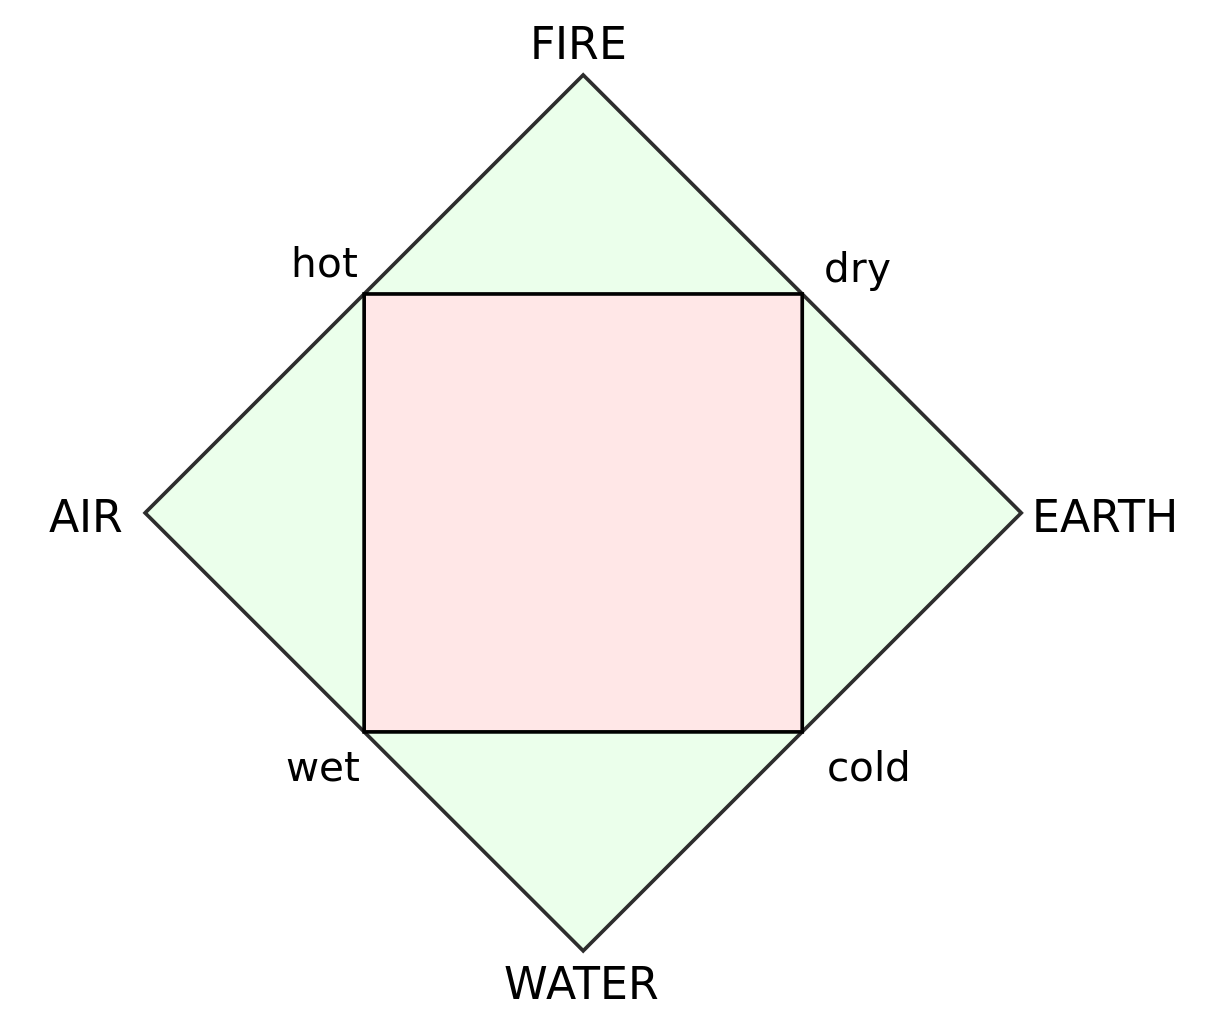
\includegraphics[width=0.90\textwidth]{figures/intro/Four_elements_representation.png}
      \end{center}
\caption{The four roots how they relate to the sensible quantities.}
\label{fig:aristotle}
\end{figure}

Today we have the Standard Model, the theoretical framework that best describes the
experimentally oberserved phenomena of the fundamental particles and their interactions. The theory
is not perfect, and it remains an overarching theme of particle physics to unify physical processes
at all energy scales under one single framework, if such a thing can be done at all.
The SM, its successes, and its shortcomings are described in
Sections~\ref{sec:SM}, \ref{sec:SMsuccess}, and \ref{sec:SMshortcomings}.

Recently in 2012, the last piece to the SM was put into place with the discovery of the Higgs boson.
This discovery, described in Section~\ref{sec:discovery}, is the foundation for the work based on
this thesis, the goal of which is to describe the first search for diHiggs production, a process
in which two Higgs bosons are produced. The motivations for what the search for this process means
in the context of SM physics and ``new'' physics is given in Section~\ref{sec:diHiggs}.

Finally, for those readers who have by chance come across this thesis and do not
have any physics training, Appendix~\ref{ch:mom} may be especially appealing.

\section{The Standard Model\label{sec:SM}}

The Standard Model (SM) of particle physics is a relativistic quantum field theory
that describes how the known fundamental particles interact through the electromagnetic, weak,
and strong forces.
The theory was developed through the unification of the electromagnetic and weak forces by Glashow
in 1961~\cite{1961.Glashow.Partial-symmetries} and through the incorporation of this electroweak
theory with the Higgs mechanism by Weinberg and Salam in 1967~\cite{PhysRevLett.19.1264,Salam:1968rm}.
This theory explained the experimental observations of the day, and later experiments provided
additional evidence as well as a mean for measuring the free parameters of the theory. Some of
this evidence is provided in Figure~\ref{fig:discoveries} in the form of the discoveries of
the fundamental particles.

\begin{figure}[ht]
 \begin{center}
    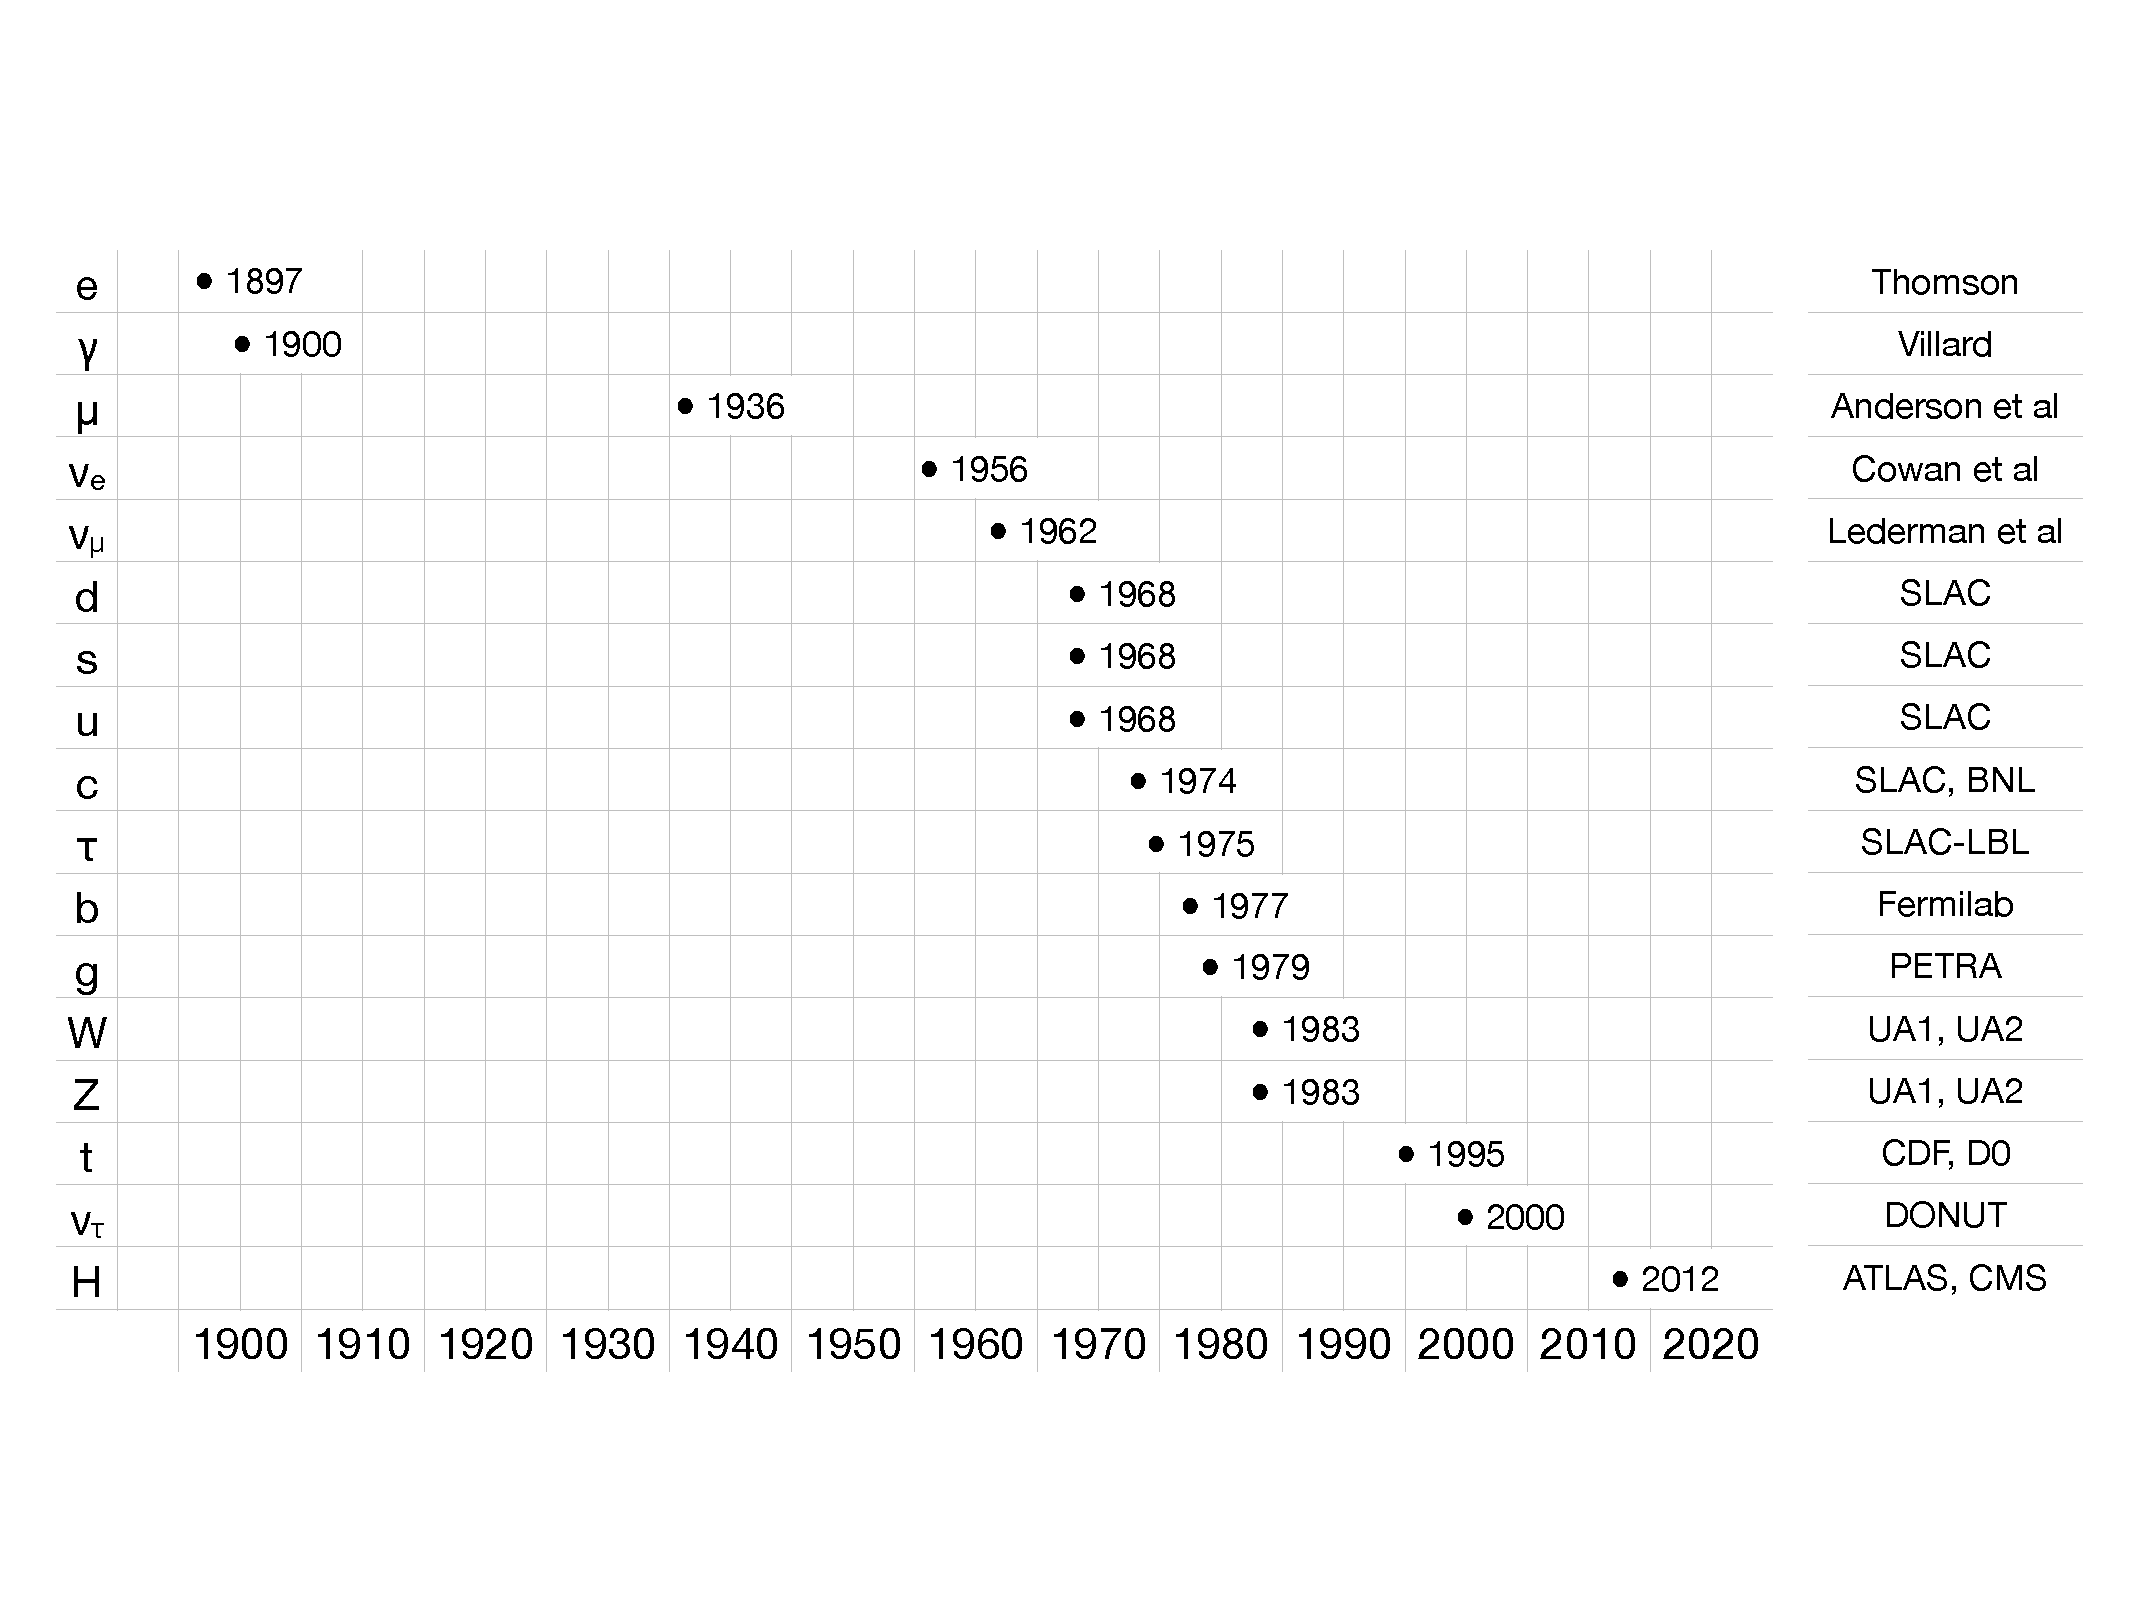
\includegraphics[width=0.90\textwidth]{figures/intro/discoveries.pdf}
      \end{center}
\caption{The discoveries of fundamental particles versus time~\cite{Tuna:thesis}.}
\label{fig:discoveries}
\end{figure}

In this theory, particles are treated as excitations of fields having half-integer spin or
integer spin, and the forces are treated as interactions among excitations of these fields.
The spin-$\frac{1}{2}$ particles, or fermions, can be divided into groups based on the ways
in which they interact. The leptons, or those particles which only experience the electroweak force,
are the electron $e$, muon $\mu$, tau $\tau$, electron neutrino $\nu_e$, muon neutrino $\nu_\mu$, and
tau neutrino $\nu_\tau$. The quarks, or those particles which experience both electoweak and strong
forces, are the up $u$, down $d$, strange $s$, charm $c$, bottom $b$, and top $top$. The integer-spin
particles, or bosons, are the spin-1 photon $\gamma$, $W$, $Z$, and gluon $g$ and the spin-0 Higgs $H$.
The particle content of the SM is summarized in Figure~\ref{fig:SMtable}.

\begin{figure}[ht]
 \begin{center}
    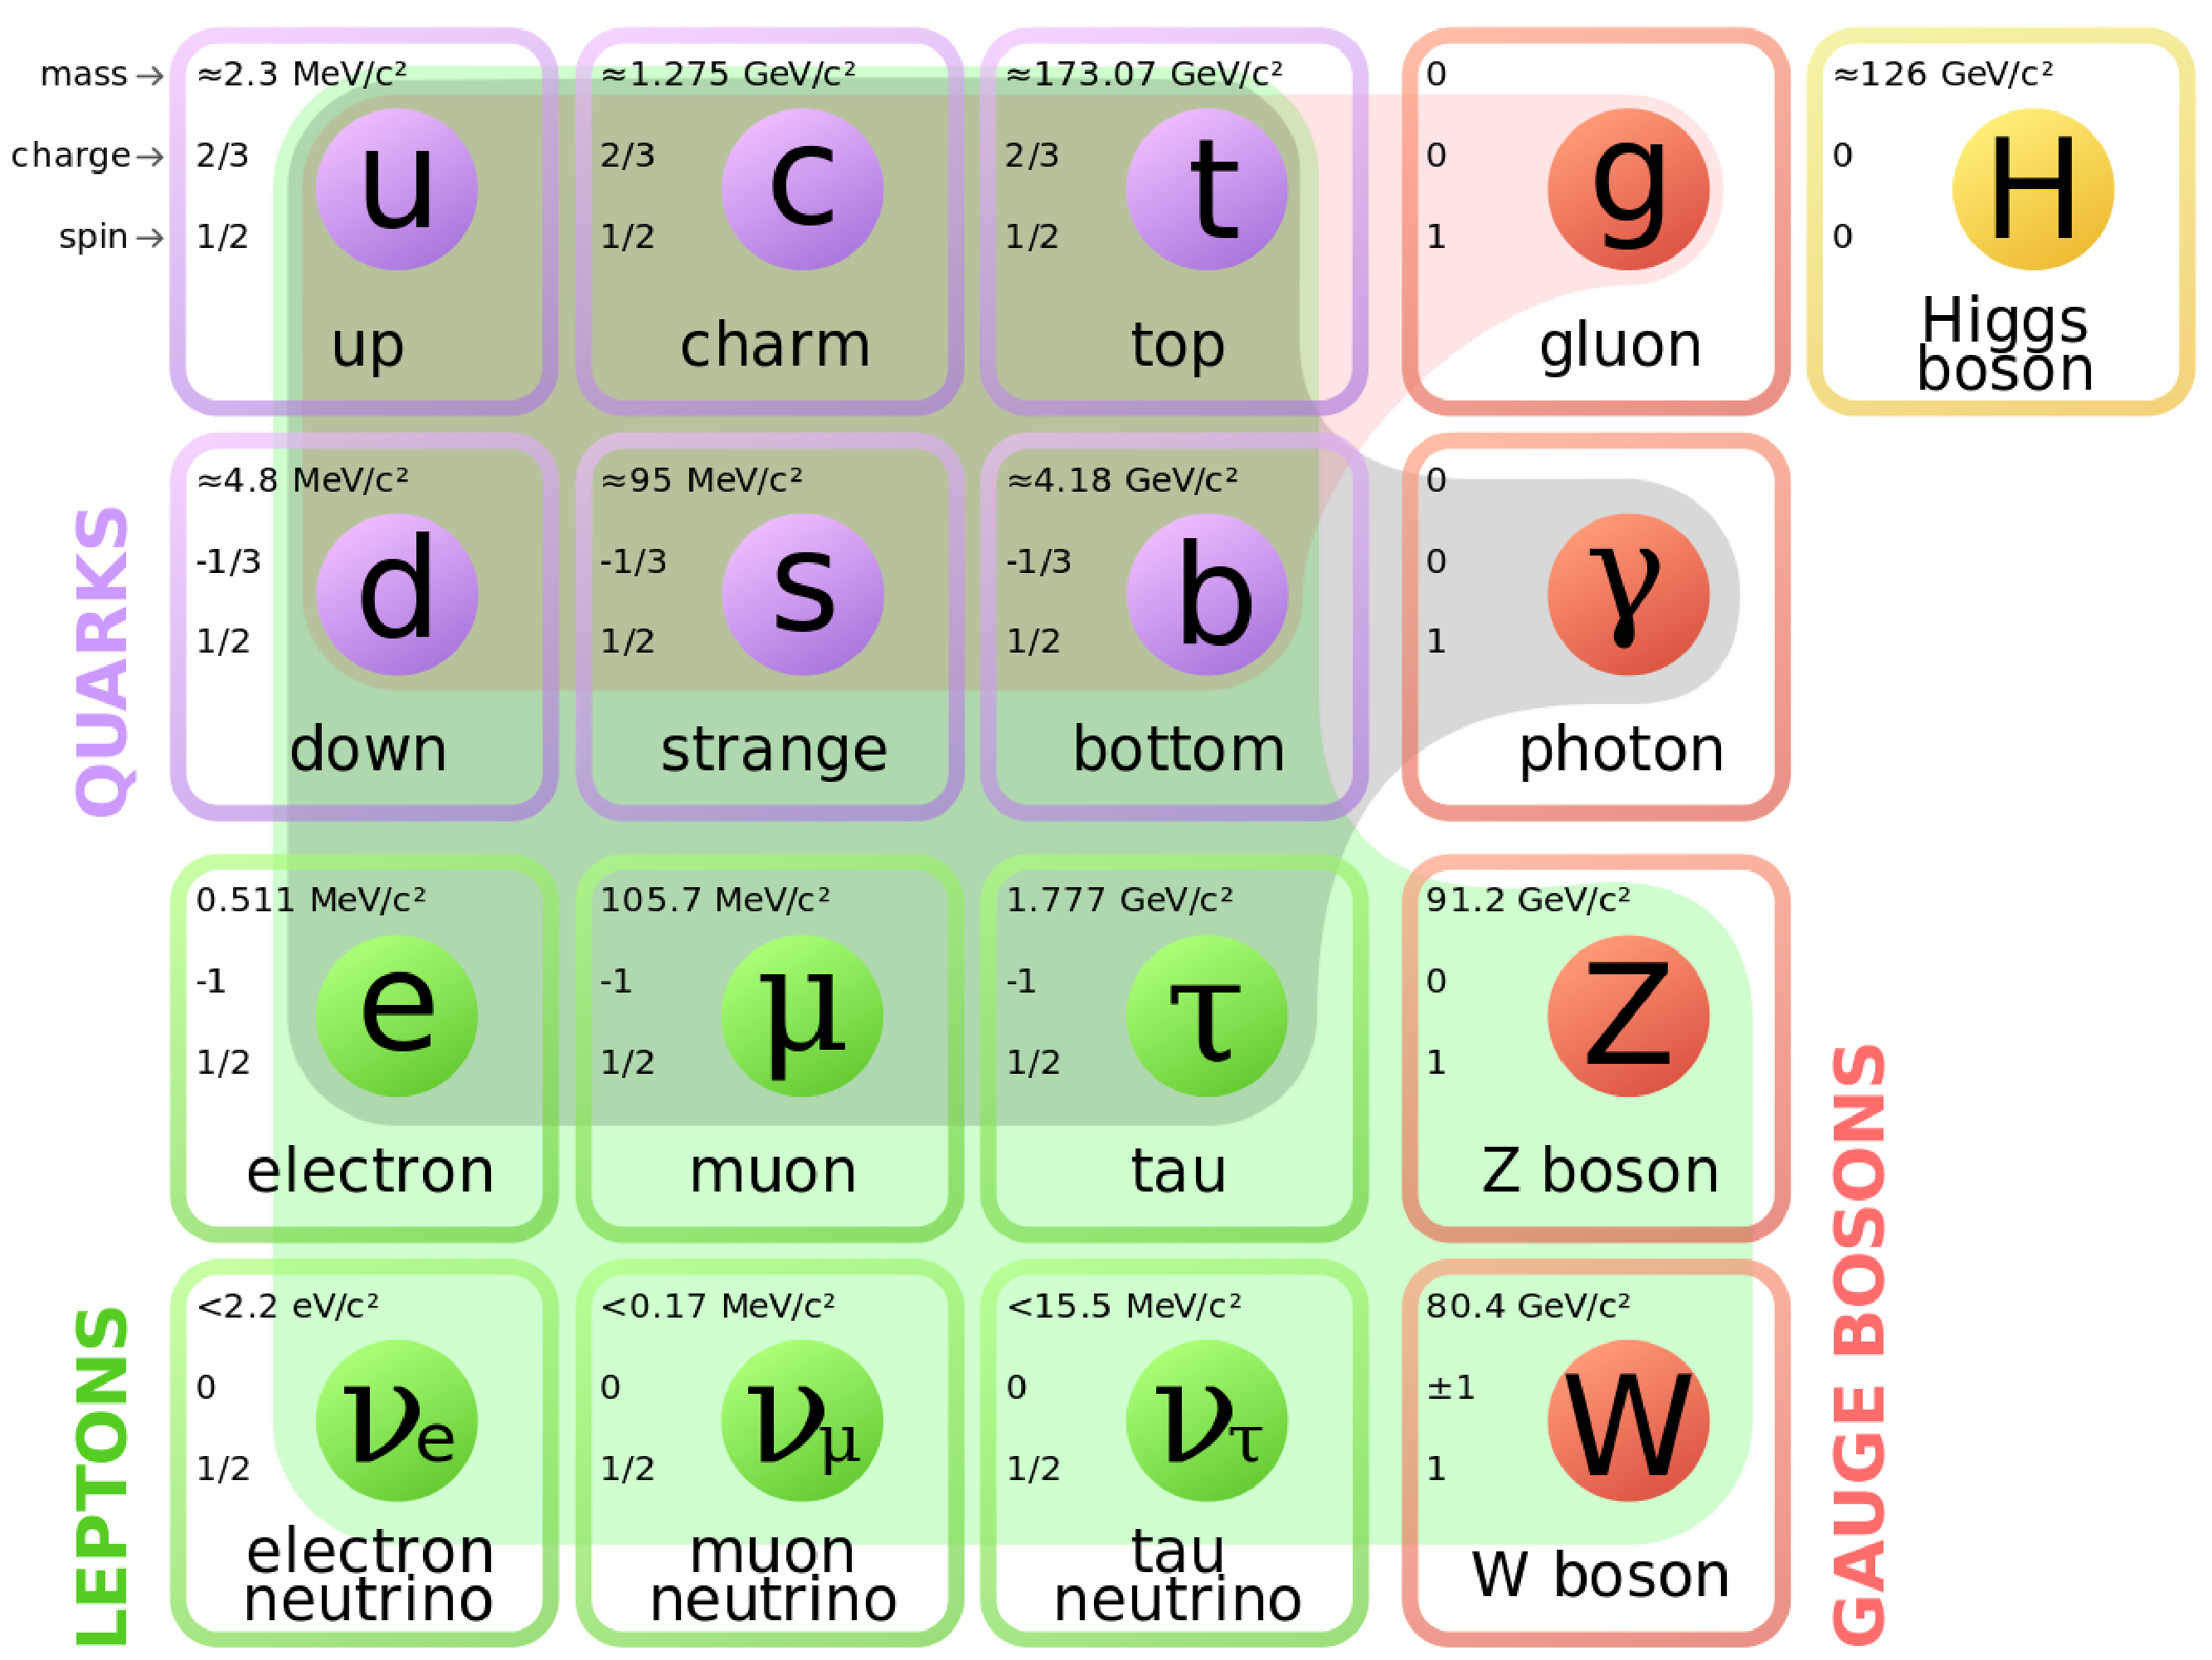
\includegraphics[width=0.90\textwidth]{figures/intro/Standard_Model_of_Elementary_Particles_modified_version.pdf}
      \end{center}
\caption{A diagram of the particle content of the SM~\cite{SMdiagram}.
The mass, electric charge, and spin is given for each, and the background color indicates how each
fermion interacts with the bosons.}
\label{fig:SMtable}
\end{figure}

The dynamics of the SM are described through its Lagrangian, which is invariant under
gauge transformations of the group $\text{SU(3)}_C \times \text{SU(2)}_L \times \text{U(1)_Y}$.
The strong force is associated with transformations under $\text{SU(3)}_C$, which give rise to
the conserved color charge $C$, denoted red, green, or blue, and eight gauge fields.
The group acts on 18 spinor fields corresponding to the quarks (six quark flavors in three colors)
and the eight gauge fields corresponding to the gluons.
The electroweak force is associated with transformations under $\text{SU(2)}_L \times \text{U(1)_Y}$,
the first part of which give rise to the conserved left-handed chirality $L$ and three gauge fields,
and the second part of which gives rise to the conserved weak hypercharge $Y$ one gauge field.
This group acts on left-handed doublets and right-handed singlets of the quarks, leptons, and
these four gauge fields. The quarks contribute nine doublets and 18 singlets, and the leptons contribute
three doublets and three singlets (as right-handed neutrinos do not exist).

The symmetry group of the SM does not allow for gauge-invariant mass terms. Instead,
the generation of particle masses is accomplished through the partial breaking of the
symmetry group by the addition of the Higgs field and potential, after which gauge-invariant
Yukawa interactions between fermions and the Higgs field naturally give fermion masses.
The Higgs field is a doublet of $\text{SU(2)}_L$. blah


\section{Higgs Discovery\label{sec:discovery}}
reference by sec:CMS

\section{Successes of the SM\label{sec:SMsuccess}}

\section{Shortcomings of the SM\label{sec:SMshortcomings}}
reference by sec:CMS


\section{diHiggs as a probe of SM and New Physics\label{sec:diHiggs}}




\chapter{Related Work\label{ch:pastwork}}

Everyone needs a chapter about related work, so here is a placeholder.

% include other files for sections of this chapter. These use the 'input' command since each section within a chapter should not start a new page.
% If you want to swap the order of sections, it is as simple as reversing the order you include them. 
%\section{Tables}
\label{sec:pastwork:tables}

Tables are also quite important. Any table that can fit entirely on one page can be a floating table. If a table is longer and will span multiple pages, a long table can be inserted in-line with the text. This is demonstrated in Table~\ref{tab:usage:options}, and explained in Appendix~\ref{ch:implementation}.

Tables that fit on one page use normal floating figures. Keep the 'p' placement option (in addition to 'h' and 't') so that if the float cannot fit in-line with the document text, it can be on a separate page by itself immediately after it is placed. Without the 'p' option, the float may get pushed to the end of the chapter, along will all other floats in the chapter that follow it.

Table~\ref{table:pastwork:publishing} lists the various options for publishing your dissertation, with costs, as of 2010. You will have to bring a check for the appropriate amount, made out to ``Princeton University Library'', when you submit your bound dissertation copies to Mudd Library, along with the appropriate forms and the electronic copy of your dissertation burned to a CD (not a DVD) as a single PDF file. (See~\cite{muddthesis2009}.)

Traditional publishing is cheaper initially and lets you earn royalties if the publisher sells many copies of your dissertation. However, most of us won't have a best-seller dissertation and most likely won't earn royalties anyway. Instead, by choosing open access publishing, your dissertation will be available online for free to anyone who is interested. I strongly advocate for open access, to maximize the impact of your research.

Your dissertation is protected by copyright regardless of whether or not you have the copyright registered. However, registration establishes a public record of your copyright claim~\cite{muddthesis2009}. ProQuest will submit the copyright registration for an extra fee (about \$55). Alternatively, you can register it yourself at the Copyright Office's website for only \$35: \url{http://www.copyright.gov/eco/}.

\begin{table}[htbp]
\centering
\caption[Thesis Publishing Options]{Thesis publishing options~\cite{mudd2009}, as of May 2010. }
\label{table:pastwork:publishing}
\begin{tabular}{p{0.3\textwidth} p{0.15\textwidth} p{0.15\textwidth} p{0.15\textwidth} p{0.15\textwidth}}
\toprule
\textbf{Publishing Method} & \textbf{Publishing Fee}
 & \textbf{Diploma Fee} & \textbf{Copyright Registration Fee} & \textbf{Total} \\
\midrule
\multicolumn{5}{c}{Traditional Publishing}\\
\midrule

Traditional without copyright registration
& 65 & 15 & -- & 80 \\[0.2em]

Traditional with copyright registration
& 65 & 15 & 55 & 135 \\[0.2em]

\midrule
\multicolumn{5}{c}{Open Access}\\
\midrule

Open access without copyright registration
& 160 & 15 & -- & 175 \\[0.2em]

Open access with copyright registration
& 160 & 15 & 55 & 230 \\

\bottomrule
\end{tabular}
\end{table}
%\section{Figures}
\label{sec:pastwork:figures}

Everyone needs floating figures in their dissertation. 

As shown in Figure~\ref{fig:pastwork:titlepage}, the Mudd Library dissertation requirements~\cite{muddthesis2009} specify additional options for formatting the title page. For example, if your thesis has multiple volumes, or to indicate the proper formatting for a master's thesis.

\begin{figure}[htb]
  \begin{center}
    
\includegraphics[width=0.9\linewidth]{ch-pastwork/figures/titlepage}
    \caption[Sample Title Page Layout]{Sample title page layout~\cite{muddthesis2009}}
    \label{fig:pastwork:titlepage}
  \end{center}
\end{figure}




\chapter{Conclusion\label{ch:conclusion}}

Some rehash of abstract and intro

\appendix % all chapters following will be labeled as appendices
\chapter{Printing and Binding\label{ch:printing}}

I might have an appendix at some point.



% Make the bibliography single spaced
\singlespacing
\bibliographystyle{plain}

% add the Bibliography to the Table of Contents
\cleardoublepage
\ifdefined\phantomsection
  \phantomsection  % makes hyperref recognize this section properly for pdf link
\else
\fi
\addcontentsline{toc}{chapter}{Bibliography}

% include your .bib file
\bibliography{bibs/thesis}

\end{document}

